\begin{figure}

\mode
<presentation>

\vspace*{-0.9cm}

\mode
<all>

\centering
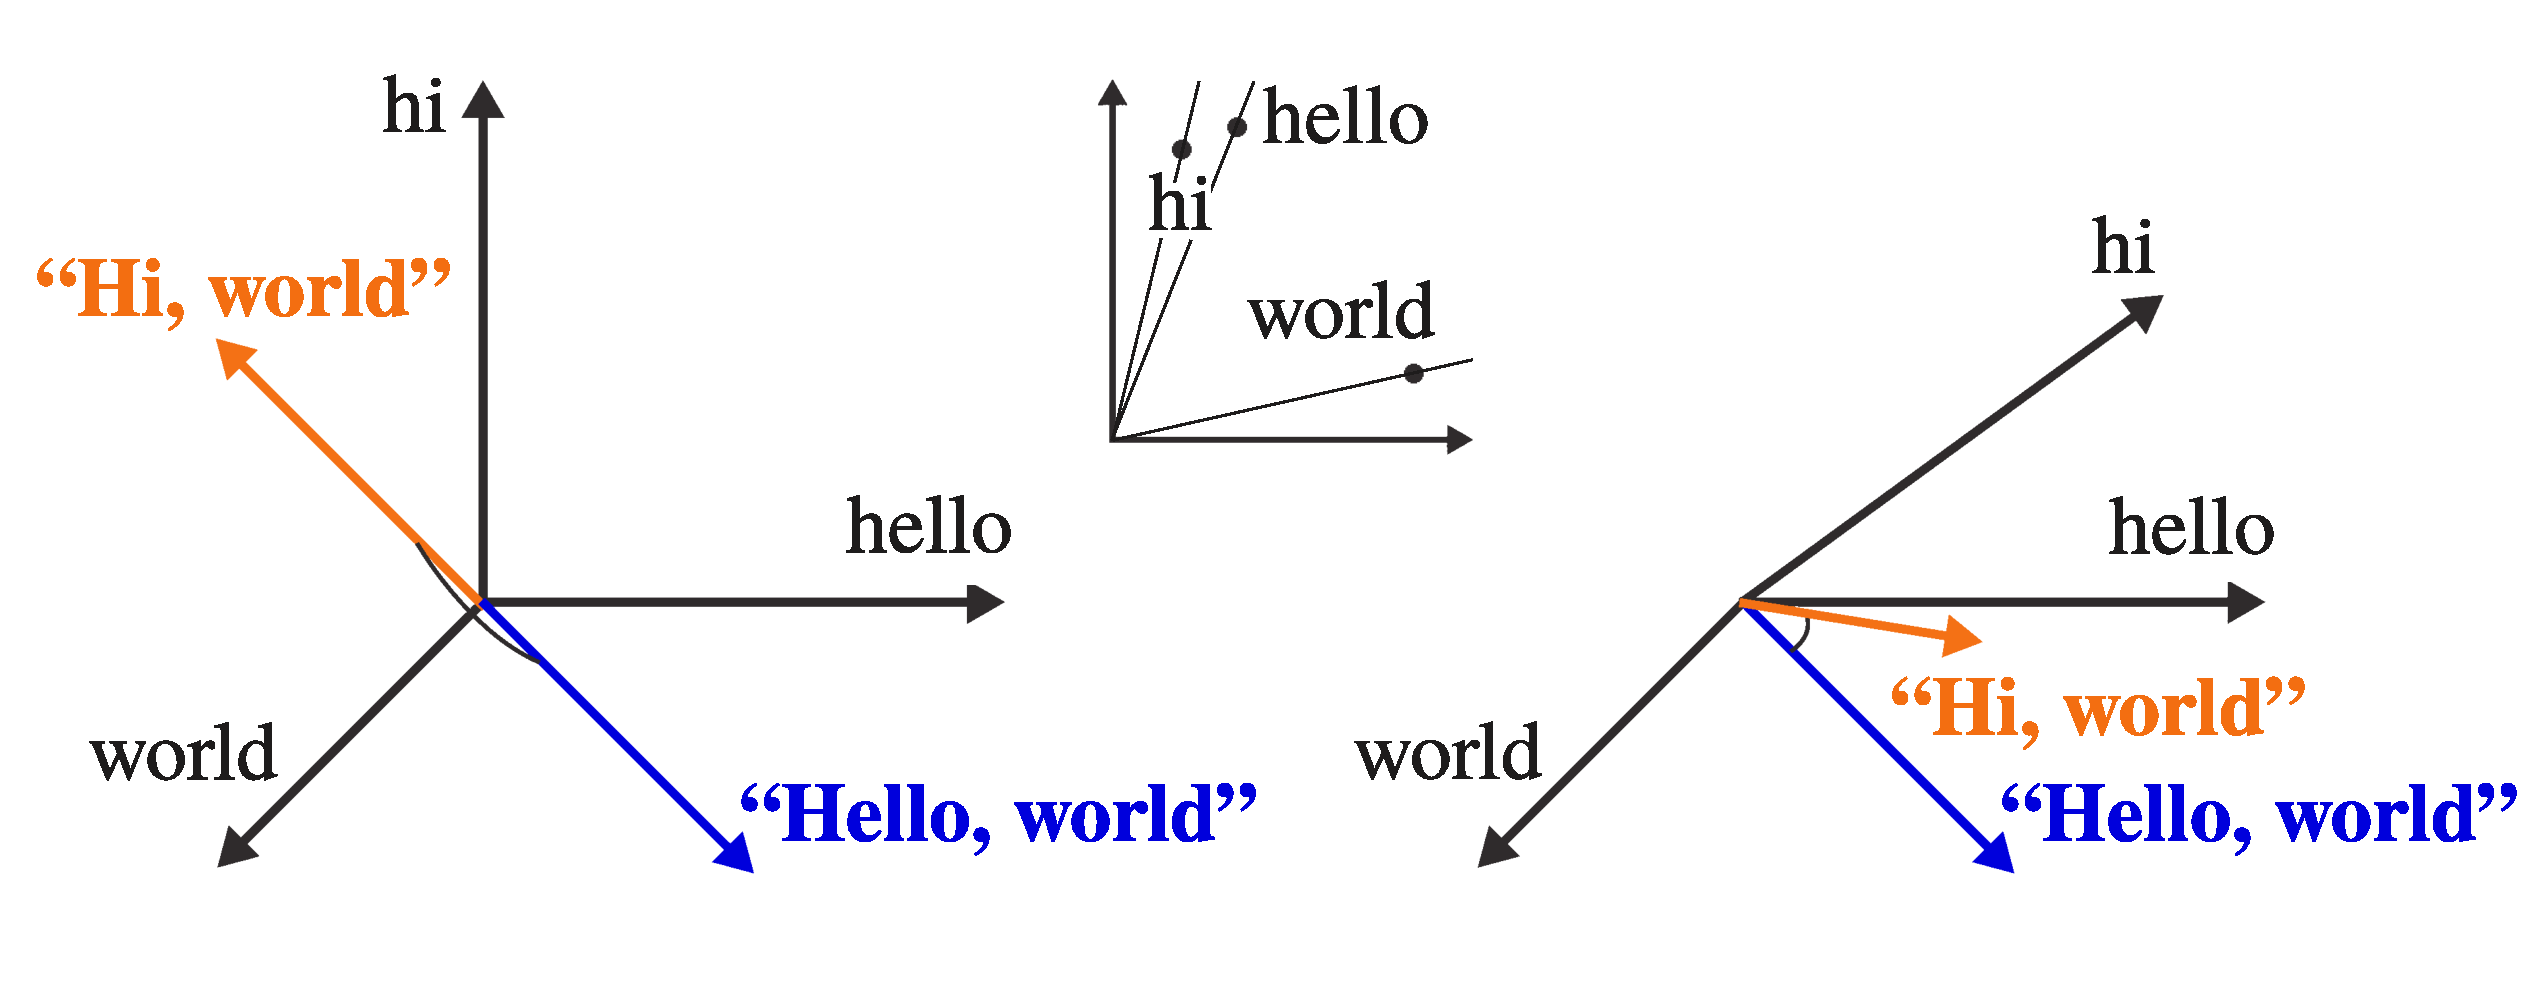
\includegraphics{soft-vsm}

\mode
<article>

\vspace{-0.4cm}

\mode
<presentation>

\vspace{-0.6cm}

\mode
<all>

\caption
  [Two sentences in hard and soft vector space models]%
  {The representations of two sentences, ``Hi, world'' and ``Hello,
   world'' in the hard vector space model (left) and in the soft vector space
   model (right). In the soft vector space model, axes are closer if the
   corresponding tokens are more related. Token embeddings (middle) can be used
   as a measure of semantic token relatedness.
   \cite[Figure 6]{novotny2020three}}
\label{fig:soft-vsm}
\end{figure}
